%\chapter{Vorlesung}
%\subsection[Laufzeit für Dinic-Algo. bei Flussnetzwerken mit Einheitskapazität]{Laufzeit für Dinic-Algorithmus bei Flussnetzwerken mit Einheitskapazität}
%\[ \mathcal{O}\left( \min\left\{ |E|^\frac{1}{2},|V|^\frac{2}{3} \right\}\cdot|E| \right) \]
\chapter{Dynamische Programmierung}
% von 9 bis 5 in 2er Gruppen, die Hälfte der Aufgaben bearbeiten, ab 16 Uhr Vorträge über letztes Blatt, Vorlesungssaal, PC-Poolräume, Seminarraum
\section{Matrizen Multiplikation}
\[ \mathbb{R}^{n\times m} \ni C = AB~~ A\in\mathbb{R}^{n\times k},~B\in\mathbb{R}^{k\times m}  \]
%Bild
\begin{figure}[H]
	\centering
	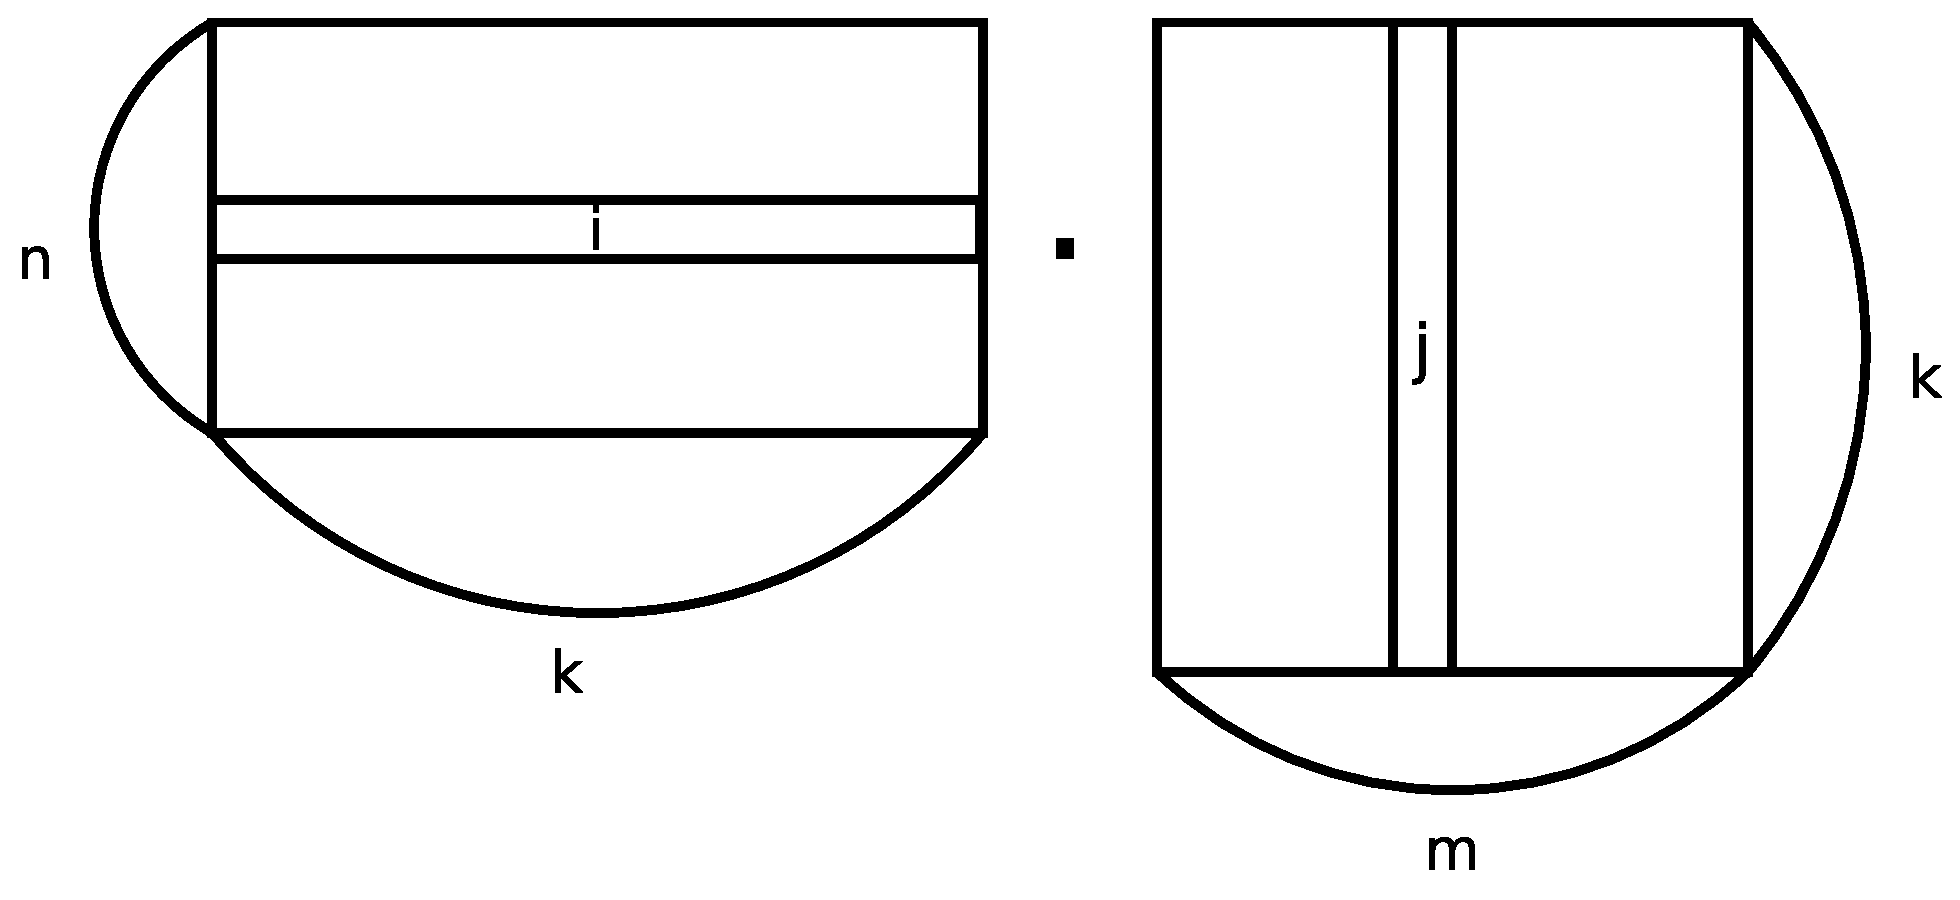
\includegraphics[width=0.5\linewidth]{29/Grafik/Diagramm1}
	\caption{Matrix-Multiplikation}
	\label{fig:Matrix-Multiplikation}
\end{figure}
\[ c_{ij} = \sum_{l = 1}^{k} a_{il}\cdot b_{li} \]
\paragraph{Laufzeit} $\mathcal{O}(n\cdot k\cdot m)$
\[ A_1\cdot A_2\cdot A_3\cdot\ldots\cdot A_n ~~~ A_i\in\mathbb{R}^{p_{i-1}\times p_i} \]
\paragraph{Beispiel}
\[ x^T\cdot a \cdot b^T \cdot y~~,a,b,x,y\in \mathbb{R}^n~~\text{Spaltenvektoren} \]
%BILD2
\begin{figure}[H]
	\centering
	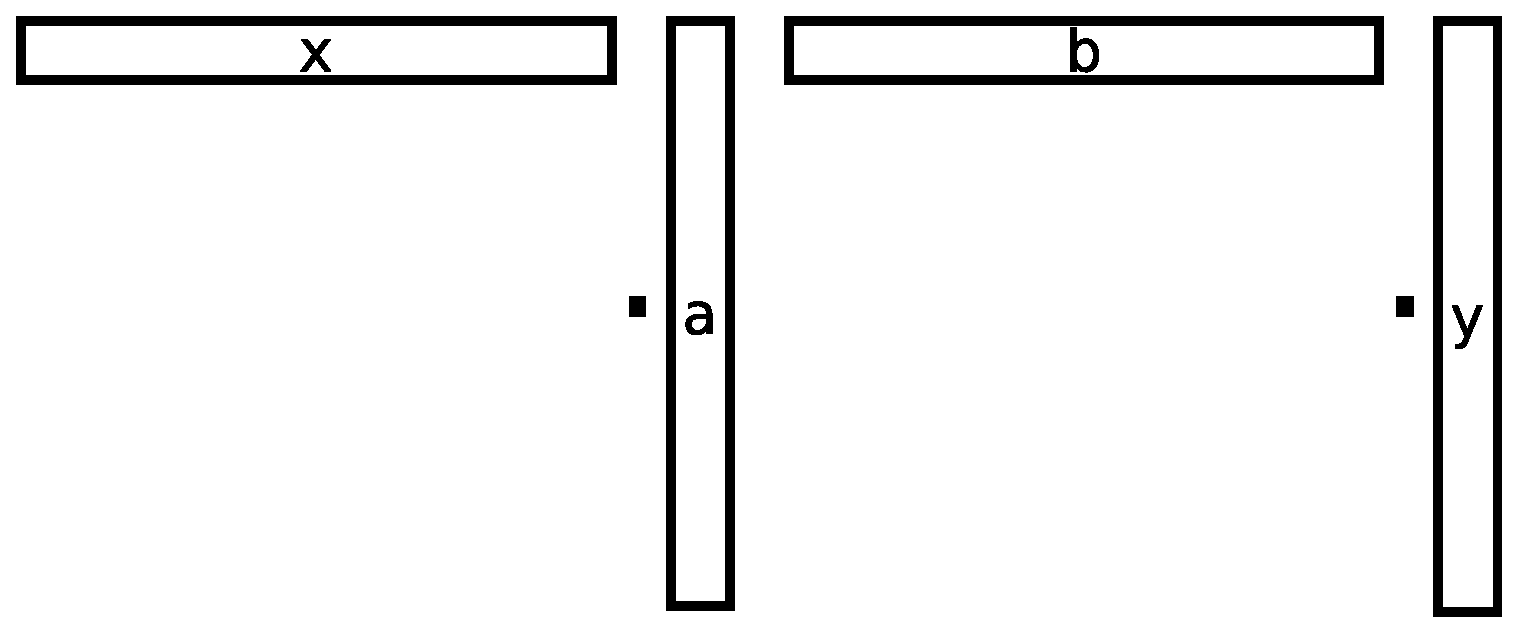
\includegraphics[width=0.4\linewidth]{29/Grafik/Diagramm2}
	\caption{Vektor-Multiplikation}
	\label{fig:Vektor-Multiplikation}
\end{figure}
\[ x^T\underset{3}{\cdot} ((a \underset{1}{\cdot} b^T) \underset{2}{\cdot} y) \]
\[ \mathbb{R}^{n\times n} \ni (a\cdot b^T) \text{ kostet }\mathcal{O}(n^2)~~~ (a\cdot b^T)\cdot y \text{ kostet } \mathcal{O} (n^2) ~~~ x^T\cdot (\ldots) \text{ kostet } \mathcal{O}(n) \]
\subparagraph{Insgesamt} $\mathcal{O}(n^2)$\\
\[ (x^T \underset{1}{\cdot} a ) \underset{3}{\cdot} (b^T \underset{2}{\cdot} y) \]
\[\mathcal{O}(n) + \mathcal{O}(1) + \mathcal{O}(n) = \mathcal{O}(n)  \]
\paragraph{Ansatz}
\[ A_1\cdot A_2\cdot A_3\cdot\ldots\cdot A_n~~~~~A_i\in\mathbb{R}^{p_{i-1}\times p_i} \]
Es gibt $C_{n-1}$ Klammerungen $C_n = \frac{1}{n+1}\binom{2n}{n}$ exponentiell in $n \in \Omega(2^n)$
\subsection{Bottom-Up Ansatz}
\[ A_{ij} = (A_i\cdot A_{i+1}\cdot\ldots\cdot A_j)\in \mathbb{R}^{p_{i-1}\times p_j} \]
\[M_{ij} = \text{ optimale Kosten zur Auswertung von} A_{ij} \]
\paragraph{Gesucht} $M_{1n}$
\[ M_{ij} = \underset{i\leq k < j}{\min} \{ M_{ik} + M_{(k+1)j} + p_{i-1}\cdot p_k\cdot p_j \}\] 
\[ M_{ii} = 0 \]
\paragraph{Nebenrechnung}
\[ A_{ij} = (A_i\cdot A_{i+1}\cdot\ldots\cdot A_k) \cdot (A_{k+2}\cdot\ldots\cdot A_j) = A_{ik} \cdot A_{(k+1)i} ~~A_{ik}\in\mathbb{R}^{p_{i-1}\times p_k},~A_{(k+1)j} \in \mathbb{R}^{p_k\times p_j} \]
\[ A_{ii} = A_i \]
\subsection{Programm}
\begin{lstlisting}[]
for (i = 1; i $\leq$ n; i++) {
	M[i][i] = 0;
}
for (l = 2; l $\leq$ n; l++) {
	for (i = 1; i $\leq$ n - l + 1; i++) {
		j = i + l - 1;
		M[i][j] = $\infty$;
		for( k = i; k < j; k++) {
			q = M[i][k] + M[k+1][k] + p[i-1] $\cdot$ p[k] $\cdot$ p[j];
			if ( q < M[i][j]) {
				M[i][j] = q;
				S[i][j] = k;
			}
		}
	}
}
\end{lstlisting}
%Muss noch nach rechts
\[ \bordermatrix {
	 &1			&2			&3			&\ldots		&j			&\ldots		& 			&n			\cr
	 &\square	&			& 			& 			&			& 			& 			& 			\cr
	i&			&\square	&\square	&\square	&\square	& 			& 			& 			\cr
	 &			&			&\square	&			&\square	&			&			&			\cr
	 &			&			&			&\square	&\square	&			&			&			\cr
	 &			&			&			&			&\square	&			&			&			\cr
	 &			&			&			&			&			&\square	&			&			\cr
	 &			&			&			&			&			&			&\square	&			\cr
	 &			&			&			&			&			&			&			&\square	\cr
} = M 
\]
\paragraph{Laufzeit} $\mathcal{O}(n^3)$